
% header %{{{1

\documentclass[tikz, border=1mm]{standalone}

\usepackage{amsmath}
\usepackage{tikz}

\usetikzlibrary{calc,angles,quotes}

\tikzset{
	% ---- default
	every path/.style={line width=0.3pt},
	every coordinate/.style={fill=black, circle, inner sep=1pt},
	every node/.style={font=\normalsize},
	every picture/.style={scale=1.0},
	% ---- custom
	construction/.style={line width=0.1pt, dashed},
	dimension/.style={line width=0.2pt, <->, goldenbrown},
	dimension extension/.style={line width=0.2pt, dashed, goldenbrown},
	vector/.style={->, thick},
}

% document %{{{1

% opening %{{{2

\begin{document}
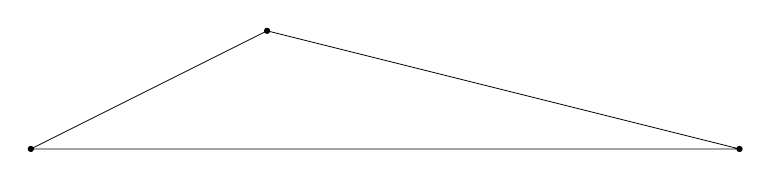
\begin{tikzpicture}[scale=1.0]

% coordinates %{{{2

	\coordinate (A) at (0,0);
	\coordinate (B) at (9,0);
	\coordinate (C) at (3,1.5);

% points, dots, vertices %{{{2

	\fill (A) circle (0.4mm);
	\fill (B) circle (0.4mm);
	\fill (C) circle (0.4mm);

% segments %{{{2

	\draw (A) -- (B) -- (C) -- cycle;

% points, dots, vertices labels %{{{2

	%\node[below left] at (A) {$A$};
	%\node[below right] at (B) {$B$};
	%\node[above] at (C) {$C$};

% segments labels %{{{2

	%\node[below]  at ($(A)!0.5!(B)$) {$c$};
	%\node[above left] at ($(A)!0.5!(C)$) {$b$};
	%\node[above right] at ($(B)!0.5!(C)$) {$a$};

% closing %{{{2

\end{tikzpicture}
\end{document}
